% ------------------------------------------------------------------------------
% TYPO3 Version 9.5 - What's New (English Version)
%
% @author	Michael Schams <schams.net>
% @license	Creative Commons BY-NC-SA 3.0
% @link		https://typo3.org/help/documentation/whats-new/
% @language	English
% ------------------------------------------------------------------------------

\documentclass[t]{beamer}

% suppress navigation bar
\beamertemplatenavigationsymbolsempty

\mode<presentation>
{
	\usetheme{typo3slides}
}

% global variables
\title{TYPO3 Version 9.5 - What's New}
\subtitle{Summary of the new features, changes and improvements}
\author{
	\centerline{Created by:}
	\centerline{Michael Schams}
}

\date{\today}

\begin{document}

% select TYPO3 Share font
\sharefont

% ------------------------------------------------------------------------------
% Title Page
% ------------------------------------------------------------------------------

\begingroup
	\setbeamercolor{normal text}{fg=white,bg=typo3orange}
	\setbeamercolor{title}{fg=white}
	\setbeamercolor{author}{fg=white}
	\setbeamertemplate{footline}[default]
	\begin{frame}
		\titlepage
	\end{frame}
\endgroup

% ------------------------------------------------------------------------------
% Table of Contents
% ------------------------------------------------------------------------------

\section*{TYPO3 Version 9.5 - What's New}
\begin{frame}[fragile]
	\frametitle

	\begin{center}
		\LARGE
			TYPO3 Version 9.5 = TYPO3 v9 LTS
		\normalsize
	\end{center}

	During a four weeks stabilization phase between the last intermediate
	version 9.4 and the new major version 9.5 (also known as "TYPO3 v9 LTS"),
	final elements of features were completed but nothing new was started.
	\newline\newline
	This is to make sure that the LTS release is robust, stable and can power
	websites of all sizes and complexities, even those with thousands of pages.
	\newline\newline
	Please see the
	\href{https://typo3.org/help/documentation/whats-new/}{TYPO3 v9 LTS slides}
	for an overview of the changes in v9 LTS.
\end{frame}

% ------------------------------------------------------------------------------

% ------------------------------------------------------------------------------
% TYPO3 Version 9.2 - What's New - Chapter "Introduction" (English Version)
%
% @author	Michael Schams <schams.net>
% @license	Creative Commons BY-NC-SA 3.0
% @link		http://typo3.org/download/release-notes/whats-new/
% @language	English
% ------------------------------------------------------------------------------
% LTXE-CHAPTER-UID:		7fdf26cc-362160ab-d6c8b905-19722b20
% LTXE-CHAPTER-NAME:	Introduction
% ------------------------------------------------------------------------------

\section{Einführung}
\begin{frame}[fragile]
	\frametitle{Einführung}

	\begin{center}\huge{Einführung}\end{center}
	\begin{center}\huge{\color{typo3darkgrey}\textbf{Fakten}}\end{center}

\end{frame}

% ------------------------------------------------------------------------------
% LTXE-SLIDE-START
% LTXE-SLIDE-UID:		3214e510-8ceda314-7689e14c-2d422661
% LTXE-SLIDE-TITLE:		TYPO3 Version 9.2 - The Facts
% ------------------------------------------------------------------------------
\begin{frame}[fragile]
	\frametitle{Einführung}
	\framesubtitle{TYPO3 Version 9.2 - Fakten}

	\begin{itemize}
		\item Veröffentlichungsdatum: 10. April 2018
		\item Releasetyp: Sprint Release
	\end{itemize}

	\begin{figure}
		
\includegraphics[width=0.95\linewidth]{Introduction/typo3-v92-banner.jpg}
	\end{figure}

\end{frame}

% ------------------------------------------------------------------------------
% LTXE-SLIDE-START
% LTXE-SLIDE-UID:		9919ea87-1d45cce7-36a77e6a-ca0598c2
% LTXE-SLIDE-TITLE:		System Requirements
% ------------------------------------------------------------------------------
\begin{frame}[fragile]
	\frametitle{Einführung}
	\framesubtitle{Systemvoraussetzungen}

	\begin{itemize}
		\item PHP Version 7.2\newline
			\smaller
				(wird möglicherweise für zukünftige Versionen auf PHP 7.1 oder 7.0 herabgesetzt)
			\normalsize

		\item PHP Einstellungen:

			\begin{itemize}
				\item \texttt{memory\_limit} >= 128M
				\item \texttt{max\_execution\_time} >= 240s
				\item \texttt{max\_input\_vars} >= 1500
				\item compilation option \texttt{-}\texttt{-disable-ipv6} must \underline{not} be used
			\end{itemize}

		\item Die meisten von \textbf{Doctrine DBAL} unterstützten Datenbankserver arbeiten auch mit TYPO3.
			Getestete DB-Engines sind zum Beispiel:
	\end{itemize}

	\begin{figure}
		
\includegraphics[width=0.70\linewidth]{Introduction/logo-databases.png}
	\end{figure}

\end{frame}

% ------------------------------------------------------------------------------
% LTXE-SLIDE-START
% LTXE-SLIDE-UID:		35a15406-7f01d16c-e43a8668-7294e2be
% LTXE-SLIDE-TITLE:		Development, Release and Maintenance Timeline
% ------------------------------------------------------------------------------
\begin{frame}[fragile]
	\frametitle{Einführung}
	\framesubtitle{Entwicklung, Veröffentlichung und Instandhaltung}

	\textbf{TYPO3 v9}

	\begin{figure}
		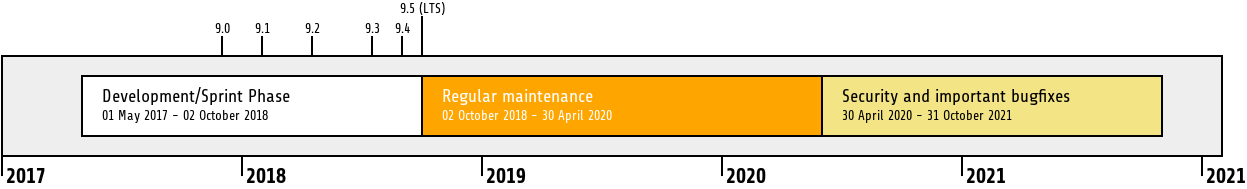
\includegraphics[width=1\linewidth]{Introduction/typo3-v9-lifecycle.png}
	\end{figure}

	\textbf{Erweiterte Unterstützung}\newline
	\smaller
		Die \href{https://typo3.com}{TYPO3 GmbH} bietet weitere Supportmöglichkeiten
		für TYPO3 v9 LTS auch nach dem 31. October 2021 für bis zu zwei weitere Jahre.
	\normalsize

%	\url{https://typo3.com/our-services/extended-support/}

\end{frame}

% ------------------------------------------------------------------------------
% LTXE-SLIDE-START
% LTXE-SLIDE-UID:		0b847921-4c7fdd13-d90d4a71-f6b1ea3a
% LTXE-SLIDE-TITLE:		TYPO3 v9 Roadmap
% ------------------------------------------------------------------------------
\begin{frame}[fragile]
	\frametitle{Einführung}
	\framesubtitle{TYPO3 v9 Roadmap}

	Voraussichtliche Veröffentlichungen und deren Hauptfokus:

	\begin{itemize}

		\item v9.0 \tabto{1.1cm}12/Dec/2017\tabto{3.4cm}Install Tool and Page Tree Refactoring,\newline
			\tabto{3.4cm}Vereinheitlichte Seitenübersetzungen
		\item v9.1 \tabto{1.1cm}30/Jan/2018\tabto{3.4cm}Redirect Handling
		\item
			\begingroup
				\color{typo3orange}
					v9.2 \tabto{1.1cm}10/Apr/2018\tabto{3.4cm}Site Configuration
			\endgroup
		\item v9.3 \tabto{1.1cm}12/Jun/2018\tabto{3.4cm}URL Routing 
		\item v9.4 \tabto{1.1cm}04/Sep/2018\tabto{3.4cm}Frontend Editing (Feature Freeze)
		\item v9.5 \tabto{1.1cm}02/Oct/2018\tabto{3.4cm}LTS Release

	\end{itemize}

	\smaller
		\url{https://typo3.org/news/article/typo3-v9-roadmap/}\newline
		\url{https://typo3.org/typo3-cms/roadmap/}
	\normalsize

\end{frame}

% ------------------------------------------------------------------------------
% LTXE-SLIDE-START
% LTXE-SLIDE-UID:		f1dbd9af-b7f82720-a1ae1511-544f2f94
% LTXE-SLIDE-TITLE:		Installation
% ------------------------------------------------------------------------------
\begin{frame}[fragile]
	\frametitle{Einführung}
	\framesubtitle{Installation}

	\begin{itemize}
		\item Empfohlene \textit{klassische} Installierungsschritte unter Linux/Mac OS X\newline
			(DocumentRoot ist beispielsweise \texttt{/var/www/site/htdocs}):
		\begin{lstlisting}
			$ cd /var/www/site
			$ wget --content-disposition get.typo3.org/9.2
			$ tar xzf typo3_src-9.2.0.tar.gz
			$ cd htdocs
			$ ln -s ../typo3_src-9.2.0 typo3_src
			$ ln -s typo3_src/index.php
			$ ln -s typo3_src/typo3
			$ touch FIRST_INSTALL
		\end{lstlisting}

		\item Symbolische Links unter Microsoft Windows:

			\begin{itemize}
				\item unter Windows XP/2000 kann \texttt{junction} benutzt werden
				\item unter Windows Vista und Windows 7 oder höher kann \texttt{mklink} benutzt werden
			\end{itemize}

	\end{itemize}
\end{frame}

% ------------------------------------------------------------------------------
% LTXE-SLIDE-START
% LTXE-SLIDE-UID:		a449e2cb-a0dd249f-277f3fe1-97c0e3fb
% LTXE-SLIDE-TITLE:		Installation using composer
% ------------------------------------------------------------------------------
\begin{frame}[fragile]
	\frametitle{Installation}
	\framesubtitle{Installation mit \texttt{composer}}

	% decrease font size for code listing
	\lstset{basicstyle=\tiny\ttfamily}

	\begin{itemize}
		\item Installation mit \textit{composer} unter Linux/Mac OS X:

			\begin{lstlisting}
				$ cd /var/www/site/
				$ composer create-project typo3/cms-base-distribution CmsBaseDistribution ^9
			\end{lstlisting}

		\item Alternativ kann man eine benutzerdefinierte \texttt{composer.json} Datei erstellen und ausführen:

			\begin{lstlisting}
				$ composer install
			\end{lstlisting}

			Weitere \texttt{composer.json} Beispielsdateien können unter \href{https://composer.typo3.org}{https://composer.typo3.org} heruntergeladen werden
			\normalsize

	\end{itemize}
\end{frame}

% ------------------------------------------------------------------------------

% ------------------------------------------------------------------------------
% TYPO3 Version 9.5 - What's New (English Version)
%
% @author	Michael Schams <schams.net>
% @license	Creative Commons BY-NC-SA 3.0
% @link		https://typo3.org/help/documentation/whats-new/
% @language	English
% ------------------------------------------------------------------------------

\section{Finalized Features}
\begin{frame}[fragile]
	\frametitle{Finalized Features}
	\begin{center}\huge{\color{typo3darkgrey}\textbf{Finalized Features}}\end{center}
\end{frame}

% ------------------------------------------------------------------------------
% #80398 - utf8mb4 on mysql by default for new instances

\begin{frame}[fragile]
	\frametitle{Finalized Features}
	\framesubtitle{\texttt{utf8mb4} on MySQL}

	% decrease font size for code listing
	\lstset{basicstyle=\tiny\ttfamily}

	\begin{itemize}
		\item New TYPO3 instances use \texttt{utf8mb4} on MySQL by default now
		\item This allows 4 byte unicode characters such as emojis
		\item Basic settings to use \texttt{utf8mb4} in file \texttt{LocalConfiguration.php}:

\begin{lstlisting}
'DB' => [
  'Connections' => [
    'Default' => [
      'driver' => 'mysqli',
      ...
      'charset' => 'utf8mb4',
      'tableoptions' => [
        'charset' => 'utf8mb4',
        'collate' => 'utf8mb4_unicode_ci',
      ],
    ],
  ],
],
\end{lstlisting}

	\end{itemize}

\end{frame}

% ------------------------------------------------------------------------------

\begin{frame}[fragile]
	\frametitle{Finalized Features}
	\framesubtitle{Search Engine Optimization (SEO)}

	\small
		The following SEO features have been added since TYPO3 version 9.3:
	\normalsize

	\begin{itemize}
		\item New
			\href{https://docs.typo3.org/typo3cms/CoreApiReference/ApiOverview/PageTitleApi/Index.html}{Page Title API}
			allows integrators and developers to influence
			what exactly is shown as the page title
		\item TYPO3 can generate
			\href{https://docs.typo3.org/typo3cms/CoreApiReference/ApiOverview/XmlSitemap/Index.html}{XML Sitemaps}
			now, with the capability to render different sitemaps per site and
			language
		\item Canonical links to pages are automatically added to prevent
			ranking penalties due to duplicate content for example
		\item In multi-language TYPO3 sites, \texttt{hreflang}-tags are added
			automatically
	\end{itemize}

\end{frame}

% ------------------------------------------------------------------------------
% #86214 - Implement static routes

\begin{frame}[fragile]
	\frametitle{Finalized Features}
	\framesubtitle{Static Routes}

	\begin{itemize}
		\item Static routes can be configured on a per site basis
		\item This allows integrators to have different \texttt{robots.txt}
			files for each site in a multi-site installation for example
		\item Routes can be configured as top level files or as path
		\item Configuration is possible in TYPO3 backend or directly in YAML
		\item Two options are currently supported:
			\begin{itemize}
				\item deliver static text
				\item resolve a TYPO3 URL
			\end{itemize}
		\item Resolving of static routes is implemented as a PSR-15 middleware
	\end{itemize}

\end{frame}

% ------------------------------------------------------------------------------
% #85829 - Implement symfony expression language for TypoScript conditions
% #86068 - Deprecate old condition syntax

\begin{frame}[fragile]
	\frametitle{Finalized Features}
	\framesubtitle{Symfony ExpressionLanguage}

	% decrease font size for code listing
	\lstset{basicstyle=\tiny\ttfamily}

	\begin{itemize}
		\item The \href{https://symfony.com/doc/current/components/expression_language/syntax.html}{Symfony ExpressionLanguage}
			component has been implemented for TypoScript conditions (frontend
			and backend)
		\item Some examples:

\begin{lstlisting}
[page["uid"] in 18..45]
# This condition matches, if current page uid is between 18 and 45
[END]

[not ("foo" matches "/bar/")]
# This condition matches, if "foo" does not match the regular expression '/bar/'
[END]

[request.getNormalizedParams().getHttpHost() == 'example.com']
# This condition matches, if current hostname is 'example.com'
[END]
\end{lstlisting}

		\item Using old condition syntax triggers a deprecation message
	\end{itemize}

\end{frame}

% ------------------------------------------------------------------------------
% #82363 - Make Extbase translation handling consistent with TypoScript

\begin{frame}[fragile]
	\frametitle{Finalized Features}
	\framesubtitle{Extbase Translation Handling}

	% decrease font size for code listing
	\lstset{basicstyle=\footnotesize\ttfamily}

	\begin{itemize}
		\item Extbase now renders translated records the same way as TypoScript
			does
		\item The new behaviour is controlled by the feature switch:

\begin{lstlisting}
config.tx_extbase.features.consistentTranslationOverlayHandling
  = 1
\end{lstlisting}

		\item The new behaviour is the default in v9 LTS (the feature switch
			will be removed in v10)
		\item Learn more about how to query data using Extbase in the
			\href{https://github.com/TYPO3/TYPO3.CMS/blob/master/typo3/sysext/core/Documentation/Changelog/9.5/Important-82363-MakeExtBaseTranslationHandlingConsistentWithTyposcript.rst}{TYPO3 documentation}

	\end{itemize}

\end{frame}

% ------------------------------------------------------------------------------
% #86422 - TypoScript getText property site

\begin{frame}[fragile]
	\frametitle{Finalized Features}
	\framesubtitle{Site Configuration in TypoScript}

	% decrease font size for code listing
	\lstset{basicstyle=\smaller\ttfamily}

	Site configuration can be accessed via \texttt{getText} property in
	TypoScript:

\begin{lstlisting}
page.10 = TEXT
page.10.data = site:base
page.10.wrap = The base URL is: |

page.20 = TEXT
page.20.data = site:customConfigKey.nested.value
page.20.wrap = The nested value is: |
\end{lstlisting}

\end{frame}

% ------------------------------------------------------------------------------

% ------------------------------------------------------------------------------
% TYPO3 Version 9.4 - What's New (German Version)
%
% @license	Creative Commons BY-NC-SA 3.0
% @link		https://typo3.org/help/documentation/whats-new/
% @language	German
% ------------------------------------------------------------------------------

\section{Veraltete/Entfernte Funktionen}
\begin{frame}[fragile]
	\frametitle{Veraltete/Entfernte Funktionen}

	\begin{center}\huge{Kapitel 4:}\end{center}
	\begin{center}\huge{\color{typo3darkgrey}\textbf{Veraltete/Entfernte Funktionen}\end{center}

\end{frame}

% ------------------------------------------------------------------------------
% #65578 - Deprecate enableConcatenateFiles
% #84414 - BackendUtility::shortcutExists
% #85858 - Deprecate GeneralUtility::clientInfo()
% #85699 - Deprecate methods in PageRepository
% #85759 - Deprecate GeneralUtility::getHostName
% #85760 - Deprecate GeneralUtility::unQuoteFilenames
% #85394 - Deprecate TYPO3\CMS\Core\Database\PdoHelper

\begin{frame}[fragile]
	\frametitle{Veraltete/Entfernte Funktionen}
	\framesubtitle{Veraltete Optionen und Funktionen (1)}

	\begin{itemize}
		\item Die folgenden zwei TypoScript-Optionen wurden als veraltet markiert:

			\begin{itemize}\smaller
                \item \texttt{config.enableConcatenateFiles}
                \item \texttt{config.concatenateJsAndCss}
            \end{itemize}

        	\smaller
				Der letzterer wurde durch \texttt{concatenateCss} bzw
					\texttt{concatenateJs} ersetzt
			\normalsize

		\item Die folgenden Methoden / Klassen wurden als veraltet markiert:

			\begin{itemize}\smaller
				\item \texttt{TYPO3\textbackslash
					CMS\textbackslash
					Backend\textbackslash
					Utility\textbackslash
					BackendUtility::shortcutExists()}

				\item \texttt{TYPO3\textbackslash
					CMS\textbackslash
					Core\textbackslash
					Utility\textbackslash
					GeneralUtility::clientInfo()}

				\item \texttt{TYPO3\textbackslash
					CMS\textbackslash
					Core\textbackslash
					Utility\textbackslash
					GeneralUtility::getHostName()}

				\item \texttt{TYPO3\textbackslash
					CMS\textbackslash
					Core\textbackslash
					Utility\textbackslash
					GeneralUtility::unQuoteFilenames()}

				\item \texttt{TYPO3\textbackslash
					CMS\textbackslash
					Frontend\textbackslash
					Page\textbackslash
					PageRepository::getRecordsByField()}

				\item \texttt{TYPO3\textbackslash
					CMS\textbackslash
					Frontend\textbackslash
					Page\textbackslash
					PageRepository::getFileReferences()}

				\item \texttt{TYPO3\textbackslash
					CMS\textbackslash
					Core\textbackslash
					Database\textbackslash
					PdoHelper}

			\end{itemize}
	\end{itemize}

\end{frame}

% ------------------------------------------------------------------------------
% #85701 - Deprecate methods in ModuleTemplate
% #85707 - Deprecate LoginFramesetController

\begin{frame}[fragile]
	\frametitle{Veraltete/Entfernte Funktionen}
	\framesubtitle{Veraltete Optionen und Funktionen (2)}

	\begin{itemize}
		\item Die folgenden Methoden / Klassen wurden als veraltet markiert:

			\begin{itemize}\smaller
				\item \texttt{TYPO3\textbackslash
					CMS\textbackslash
					Backend\textbackslash
					Template\textbackslash
					ModuleTemplate::icons()}

				\item \texttt{TYPO3\textbackslash
					CMS\textbackslash
					Backend\textbackslash
					Template\textbackslash
					ModuleTemplate::loadJavascriptLib()}

			\end{itemize}

		\item Folgende Klasse wurde als veraltet markiert und die Funktionalität der Klasse wurde durch eine
			Anfrage an \texttt{index.php?loginRefresh=1} ersetzt:
			
			\begin{itemize}\smaller
				\item \texttt{TYPO3\textbackslash
					CMS\textbackslash
					Backend\textbackslash
					Controller\textbackslash
					LoginFramesetController}
			\end{itemize}\smaller

	\end{itemize}

\end{frame}

% ------------------------------------------------------------------------------
% #85793 - Deprecate several constants from SystemEnvironmentBuilder

\begin{frame}[fragile]
	\frametitle{Veraltete/Entfernte Funktionen}
	\framesubtitle{Veraltete Konstanten (1)}

	\begin{itemize}
		\item Folgende Konstanten sind veraltet (1/2)\newline
			und sollten nicht mehr verwendet werden:

			\begin{itemize}\smaller
				\item \texttt{TYPO3\_URL\_MAILINGLISTS}
				\item \texttt{TYPO3\_URL\_DOCUMENTATION}
				\item \texttt{TYPO3\_URL\_DOCUMENTATION\_TSREF}
				\item \texttt{TYPO3\_URL\_DOCUMENTATION\_TSCONFIG}
				\item \texttt{TYPO3\_URL\_CONSULTANCY}
				\item \texttt{TYPO3\_URL\_CONTRIBUTE}
				\item \texttt{TYPO3\_URL\_SECURITY}
				\item \texttt{TYPO3\_URL\_DOWNLOAD}
				\item \texttt{TYPO3\_URL\_SYSTEMREQUIREMENTS}
			\end{itemize}

	\end{itemize}

\end{frame}

% ------------------------------------------------------------------------------
% #85793 - Deprecate several constants from SystemEnvironmentBuilder
% #85285 - Replace last occurrences of PATH_site with Environment API

\begin{frame}[fragile]
	\frametitle{Veraltete/Entfernte Funktionen}
	\framesubtitle{Veraltete Konstanten (2)}

	\begin{itemize}
		\item Folgende Konstanten sind veraltet(2/2)\newline
			und sollten nicht mehr verwendet werden:

			\begin{itemize}\smaller
				\item \texttt{NUL}\tabto{3cm}(use \texttt{"\textbackslash 0"} instead)
				\item \texttt{TAB}\tabto{3cm}(use \texttt{"\textbackslash t"} instead)
				\item \texttt{SUB}\tabto{3cm}(use \texttt{chr(26)} instead)
				\item \texttt{PATH\_thisScript}\tabto{3cm}(use \texttt{Environment::getCurrentScript()} instead)
				\item \texttt{PATH\_site}\tabto{3cm}(use \texttt{Environment::getPublicPath().'/'} instead)
			\end{itemize}
	\end{itemize}

\end{frame}

% ------------------------------------------------------------------------------
% #85878 - Deprecate EidUtility and methods within TSFE

\begin{frame}[fragile]
	\frametitle{Veraltete/Entfernte Funktionen}
	\framesubtitle{\texttt{EidUtility} Klasse und \texttt{TSFE} Methoden}

	% decrease font size for code listing
	\lstset{basicstyle=\tiny\ttfamily}

	\begin{itemize}
		\item Folgende Klasse wurde als veraltet markiert:\newline
			\smaller\texttt{TYPO3\textbackslash
				CMS\textbackslash
				Frontend\textbackslash
				Utility\textbackslash
				EidUtility}\normalsize

		\item Folgende Methoden wurden als veraltet markiert:\newline
			\smaller\texttt{TYPO3\textbackslash
				CMS\textbackslash
				Frontend\textbackslash
				Controller\textbackslash
				TypoScriptFrontendController}\normalsize

				\begin{itemize}\smaller
					\item \texttt{TypoScriptFrontendController::initFEuser()}
					\item \texttt{TypoScriptFrontendController::storeSessionData()}
					\item \texttt{TypoScriptFrontendController::previewInfo()}
					\item \texttt{TypoScriptFrontendController::hook\_eofe()}
					\item \texttt{TypoScriptFrontendController::addTempContentHttpHeaders()}
					\item \texttt{TypoScriptFrontendController::sendCacheHeaders()}
				\end{itemize}

			\item Folgender Hook wurde als veraltet markiert:

				\begin{lstlisting}
$GLOBALS['TYPO3_CONF_VARS']['SC_OPTIONS']['tslib/class.tslib_fe.php']['hook_previewInfo']
				\end{lstlisting}

	\end{itemize}

\end{frame}

% ------------------------------------------------------------------------------
% #85004 - Deprecate methods in ReflectionService

\begin{frame}[fragile]
	\frametitle{Veraltete/Entfernte Funktionen}
	\framesubtitle{Die Klasse \texttt{ReflectionService}}

	\begin{itemize}
		\item Folgende Methoden wurden als veraltet markiert:\newline
			\smaller\texttt{TYPO3\textbackslash
				CMS\textbackslash
				Extbase\textbackslash
				Reflection\textbackslash
				ReflectionService}\normalsize

				\begin{itemize}\smaller
					\item \texttt{ReflectionService::getClassTagsValues()}
					\item \texttt{ReflectionService::getClassTagValues()}
					\item \texttt{ReflectionService::getClassPropertyNames()}
					\item \texttt{ReflectionService::hasMethod()}
					\item \texttt{ReflectionService::getMethodTagsValues()}
					\item \texttt{ReflectionService::getMethodParameters()}
					\item \texttt{ReflectionService::getPropertyTagsValues()}
					\item \texttt{ReflectionService::getPropertyTagValues()}
					\item \texttt{ReflectionService::isClassTaggedWith()}
					\item \texttt{ReflectionService::isPropertyTaggedWith()}
				\end{itemize}

	\end{itemize}

\end{frame}

% ------------------------------------------------------------------------------
% More functions have been deprecated/removed...

\begin{frame}[fragile]
	\frametitle{Veraltete/Entfernte Funktionen}

	\vspace{0.6cm}
	\begin{center}
		Viele weitere Funktionen
	\end{center}
	\vspace{-0.8cm}
	\begin{center}
		wurden in der TYPO3 Version 9.4
	\end{center}
	\vspace{-0.8cm}
	\begin{center}
		als veraltet markiert oder entfernt.
	\end{center}
	\vspace{-0.6cm}
	\begin{center}
		Bitte die
\href{https://docs.typo3.org/typo3cms/extensions/core/latest/Changelog/9.4/Index.html#deprecation}{TYPO3 Dokumentation} prüfen für weitere Informationen.
	\end{center}

\end{frame}

% ------------------------------------------------------------------------------

% ------------------------------------------------------------------------------
% TYPO3 Version 9.1 - What's New - Chapter "Sources" (English Version)
%
% @author	Michael Schams <schams.net>
% @license	Creative Commons BY-NC-SA 3.0
% @link		http://typo3.org/download/release-notes/whats-new/
% @language	English
% ------------------------------------------------------------------------------
% LTXE-CHAPTER-UID:		b28441c6-44c982a3-35fcefd3-f4dc5d5c
% LTXE-CHAPTER-NAME:	Sources and Authors
% ------------------------------------------------------------------------------

\section{Quellen und Autoren}
\begin{frame}[fragile]
	\frametitle{Quellen und Autoren}

	\begin{center}\huge{Kapitel 6:}\end{center}
	\begin{center}\huge{\color{typo3darkgrey}\textbf{Quellen und Autoren}}\end{center}

\end{frame}

% ------------------------------------------------------------------------------
% LTXE-SLIDE-START
% LTXE-SLIDE-UID:		51b2cb0b-b390885b-49e40a7d-63be1365
% LTXE-SLIDE-TITLE:		Sources
% ------------------------------------------------------------------------------

\begin{frame}[fragile]
	\frametitle{Quellen und Autoren}
	\framesubtitle{Quellen}

	\textbf{TYPO3 News:}
		\begin{itemize}\smaller
			\item \url{https://typo3.org/news}
		\end{itemize}

	\textbf{Release Infos:}
		\begin{itemize}\smaller
			\item \url{https://get.typo3.org/release-notes/9.x/TYPO3_CMS_9.1.0}
			\item \href{https://github.com/TYPO3/TYPO3.CMS/blob/master/INSTALL.md}{INSTALL.md}
				und \href{https://github.com/TYPO3/TYPO3.CMS/tree/master/typo3/sysext/core/Documentation/Changelog}{ChangeLog}
			\item \texttt{typo3/sysext/core/Documentation/Changelog/9.1/*}
		\end{itemize}

	\textbf{TYPO3 Bug-/Issuetracker:}
		\begin{itemize}\smaller
			\item \url{https://forge.typo3.org/projects/typo3cms-core}
		\end{itemize}

	\textbf{TYPO3 und Fluid Git Repositories:}
		\begin{itemize}\smaller
			\item \url{https://git.typo3.org/Packages/TYPO3.CMS.git}
			\item \url{https://github.com/TYPO3/Fluid}
		\end{itemize}

\end{frame}

% ------------------------------------------------------------------------------
% LTXE-SLIDE-START
% LTXE-SLIDE-UID:		98970217-deba22a1-cd6ec09f-b8d5e671
% LTXE-SLIDE-TITLE:		Authors
% ------------------------------------------------------------------------------

\begin{frame}[fragile]
	\frametitle{Quellen und Autoren}

	\vspace{-0.6cm}

	\centerline{\textbf{TYPO3 CMS What's New Team:}}

	\begin{center}
		\centerline{Pierrick Caillon, Richard Haeser, Jigal van Hemert}
		\centerline{Henrietta Kucsovan, Michael Schams and Roberto Torresani}
	\end{center}

	\vspace{0.8cm}

	\smaller\begin{center}\url{https://typo3.org/download/release-notes/whats-new}\end{center}\normalsize

	\vspace{1cm}

	\smaller\begin{center}Licensed under Creative Commons BY-NC-SA 3.0\end{center}\normalsize
	\begin{figure}\vspace*{-0.4cm}
		
\includegraphics[width=1.4cm]{SourcesAndAuthors/CreativeCommons-BY-NC-SA.png}
	\end{figure}

\end{frame}

% ------------------------------------------------------------------------------


% ------------------------------------------------------------------------------

%% ------------------------------------------------------------------------------
% TYPO3 - What's New - Test/Example Chapter
%
% @license	Creative Commons BY-NC-SA 3.0
% @link		https://typo3.org/help/documentation/whats-new/
% @language	Italian
% ------------------------------------------------------------------------------
% Test/Example Chapter
% ------------------------------------------------------------------------------

\section{Test Chapter}
\begin{frame}[fragile]
	\frametitle{Test Chapter}

	\begin{center}\huge{Test Chapter:}\end{center}
	\begin{center}\huge{\color{typo3darkgrey}\textbf{LaTeX Styles, Formatting, etc.}}\end{center}

\end{frame}

% ------------------------------------------------------------------------------
% Example: Font Styles (Formatting)
% ------------------------------------------------------------------------------

\begin{frame}
	\frametitle{Test Chapter}
	\framesubtitle{Font Styles}

	\begin{itemize}
		\item \emph{emphasis}
		\item \textsf{Sans}
		\item \texttt{teletypefont}
		\item \textit{italic}
		\item \underline{underline}
		\item \uppercase{uppercase}
		\item \textbf{bold}
		\item \alert{alert}
		\item
			\begingroup
				\color{typo3orange}
				typo3orange
			\endgroup

	\end{itemize}

\end{frame}

% ------------------------------------------------------------------------------
% Example: Links And Levels
% ------------------------------------------------------------------------------

\begin{frame}
	\frametitle{Test Chapter}
	\framesubtitle{Links}

	\begin{itemize}
		\item Item
		\item Item with link: \url{https://example.com}
		\item Item with \href{https://example.com}{link label}

		\item First level
		\begin{itemize}
			\item Second level
			\begin{itemize}
				\item Third level
			\end{itemize}
		\end{itemize}

	\end{itemize}

\end{frame}

% ------------------------------------------------------------------------------
% Example: Item List
% ------------------------------------------------------------------------------

\begin{frame}
	\frametitle{Test Chapter}
	\framesubtitle{Item List}

	\begin{itemize}
		\item Item 1
		\item Item 2
		\item Item 3
		\item Item 4
		\item Item 5
		\item Item 6
		\item Item 7
		\item Item 8
		\item Item 9
		\item Item 10
		\item Item 11
		\item Item 12
	\end{itemize}

\end{frame}

% ------------------------------------------------------------------------------
% Example: Two Columns
% ------------------------------------------------------------------------------

\begin{frame}
	\frametitle{Test Chapter}
	\framesubtitle{Two Columns}

	\begin{columns}[T]

		\begin{column}{.5\textwidth}
			\begin{itemize}
				\item Item 1
				\item Item 2
				\item Item 3
				\item Item 4
				\item Item 5
				\item Item 6
			\end{itemize}
		\end{column}

		\begin{column}{.5\textwidth}
			\begin{itemize}
				\item Item 7
				\item Item 8
				\item Item 9
				\item Item 10
				\item Item 11
				\item Item 12
			\end{itemize}
		\end{column}

	\end{columns}

\end{frame}

% ------------------------------------------------------------------------------
% Example: Code Snippet
% ------------------------------------------------------------------------------

\begin{frame}[fragile]
	\frametitle{Test Chapter}
	\framesubtitle{Code Snippets}

	\begin{itemize}
		\item code outside a bullet list:
	\end{itemize}

	\begin{lstlisting}
		page = PAGE
		page.10 = TEXT
		page.10.value = Hello World
	\end{lstlisting}

	\begin{itemize}
		\item code inside a bullet list (indented):
		\begin{lstlisting}
			page = PAGE
			page.10 = TEXT
			page.10.value = Hello World
		\end{lstlisting}
	\end{itemize}

	\begin{itemize}
		\item inline code: \lstinline!var i:integer;!
		\item inline code: \texttt{var i:integer}
	\end{itemize}

\end{frame}

% ------------------------------------------------------------------------------
% Example: Code Snippet
% ------------------------------------------------------------------------------

\begin{frame}[fragile]
	\frametitle{Test Chapter}
	\framesubtitle{Code Snippets}

	\begin{itemize}
		\item custom font sizes (if not avoidable):

		\lstset{
			basicstyle=\large\selectfont\ttfamily
		}

		\begin{lstlisting}
			page = PAGE
			page.10 = TEXT
			page.10.value = Hello World
		\end{lstlisting}

		\lstset{
			basicstyle=\small\selectfont\ttfamily
		}

		\begin{lstlisting}
			page = PAGE
			page.10 = TEXT
			page.10.value = Hello World
		\end{lstlisting}

		\lstset{
			basicstyle=\fontsize{7}{9}\selectfont\ttfamily
		}

		\begin{lstlisting}
			page = PAGE
			page.10 = TEXT
			page.10.value = Hello World
		\end{lstlisting}

		\lstset{
			basicstyle=\tiny\ttfamily
		}

		\begin{lstlisting}
			page = PAGE
			page.10 = TEXT
			page.10.value = Hello World
		\end{lstlisting}

	\end{itemize}

%	\tabto{1cm} \texttt{custom indentation: 1cm from left}\newline
%	\tabto{1.5cm} \texttt{custom indentation: 1.5cm from left}\newline
%	\tabto{2cm} \texttt{custom indentation: 2cm from left}\newline
%	\tabto{2.5cm} \texttt{custom indentation: 2.5cm from left}\newline

\end{frame}

% ------------------------------------------------------------------------------
% Example: Slide Without Bullet Points
% ------------------------------------------------------------------------------

\begin{frame}
	\frametitle{Test Chapter}
	\framesubtitle{A Slide Without Bullet Points}

	Lorem ipsum dolor sit amet, consectetur adipisicing elit, sed do eiusmod
	tempor incididunt ut labore et dolore magna aliqua. Ut enim ad minim veniam,
	quis nostrud exercitation ullamco laboris nisi ut aliquip ex ea commodo
	consequat. Duis aute irure dolor in reprehenderit in voluptate velit esse
	cillum dolore eu fugiat nulla pariatur. Excepteur sint occaecat cupidatat
	non proident, sunt in culpa qui officia deserunt mollit anim id est laborum.

	%\breakingchange{BREAKING CHANGE!}
	\breakingchange

\end{frame}

% ------------------------------------------------------------------------------
% Example: Text Sizes
% ------------------------------------------------------------------------------

\begin{frame}
	\frametitle{Test Chapter}
	\framesubtitle{Text Sizes}

	\begin{itemize}
		\item Default text size ("normalsize"):\newline
			Lorem ipsum dolor sit amet, consectetur adipisicing elit, sed do eiusmod tempor incididunt ut labore et dolore magna aliqua.

		\item Small text size:\newline
			\small
				Lorem ipsum dolor sit amet, consectetur adipisicing elit, sed do eiusmod tempor incididunt ut labore et dolore magna aliqua.
			\normalsize

		\item Smaller text size:\newline
			\smaller
				Lorem ipsum dolor sit amet, consectetur adipisicing elit, sed do eiusmod tempor incididunt ut labore et dolore magna aliqua.
			\normalsize

		\item Tiny text size:\newline
			\tiny
				Lorem ipsum dolor sit amet, consectetur adipisicing elit, sed do eiusmod tempor incididunt ut labore et dolore magna aliqua.
			\normalsize

	\end{itemize}
\end{frame}

% ------------------------------------------------------------------------------


% ------------------------------------------------------------------------------
\end{document}
